\section{Research Questions}
Our research questions aim to discover how people perceive and discuss armed conflicts. We suspect some of the same biases that affect traditional media will also affect social media, especially Reddit due to its news-driven process. However, it is unlikely there will be complete overlap.

Our data set consists of approximately 426GB of Reddit data, ranging from the year 2012 to the year 2014. We cross-referenced this with data from the Armed Conflicts Database, collecting a list of 48 conflicts that are considered by the Database to have been active in at least one of those years. This was to ensure none of the conflicts were seen by commenters as purely historical. See Figure~\ref{conflicts} for a summary of where the conflicts occurred. 

We gathered Reddit comments that are relevant to each of the 48 conflicts by searching for comments in every single subreddit. We compiled sets of keywords for every conflict then collected comments which matched them. For instance, if a comment contained the phrase ``Syrian Civil War'' (not case-sensitive), we would mark that comment as relevant to the conflict in Syria. While there are certainly some false positives, we sought to counter that by having a sufficiently large data set. The biggest source of comments was the ``worldnews'' subreddit, with many of the others coming from similar subreddits. We took this as positive evidence that the majority of our comments were on topic. 

\begin{figure}
\centering
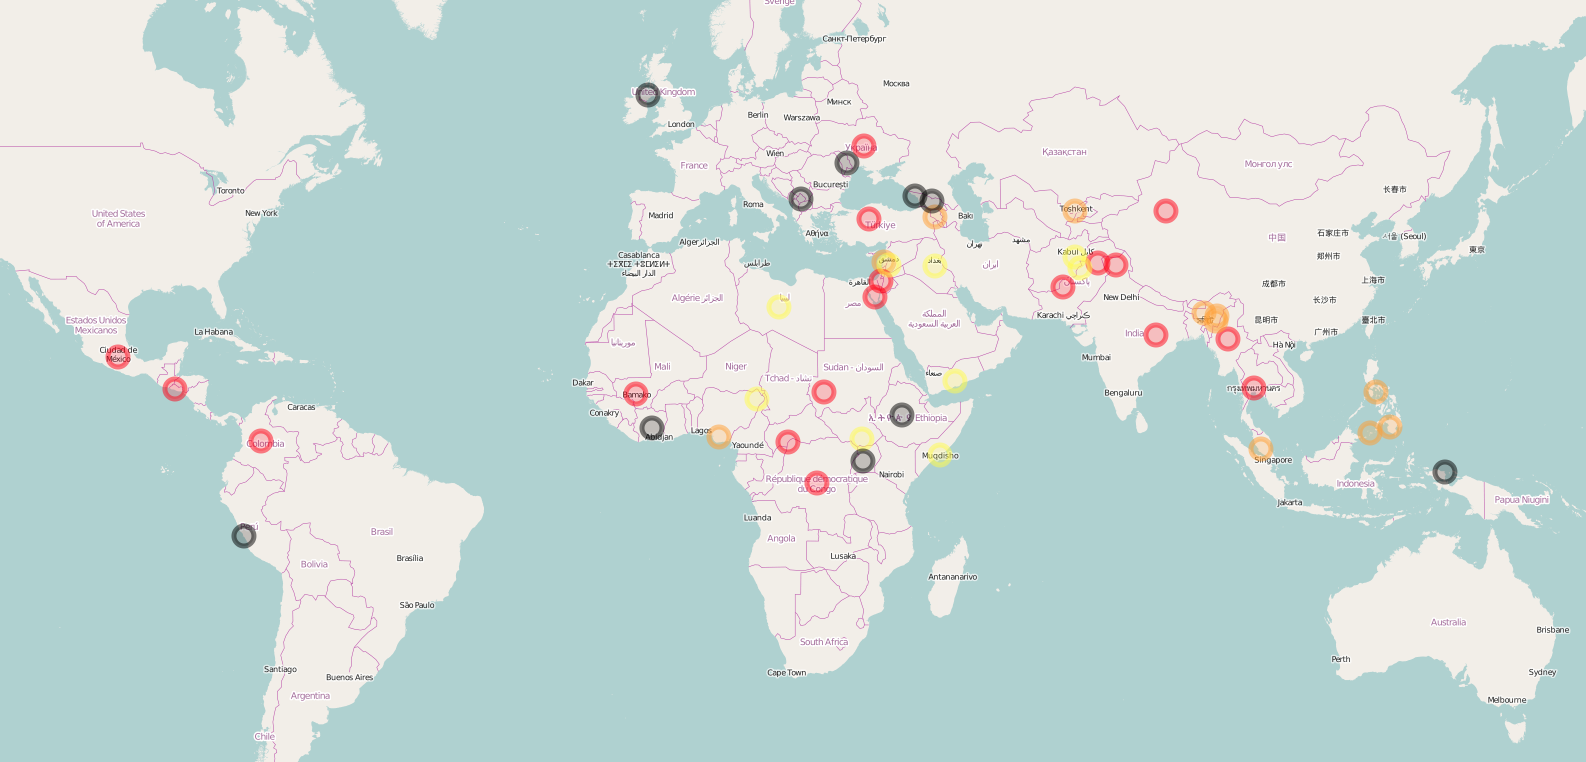
\includegraphics[width=0.9\columnwidth]{map}
\caption{A map of the 48 conflicts. Black, yellow, orange and red circles indicate the current level of intensity as rated by the Armed Conflict Database: archived, low, medium and high, respectively.}
\label{conflicts}
\end{figure}